\documentclass{article}%
\usepackage[T1]{fontenc}%
\usepackage[utf8]{inputenc}%
\usepackage{lmodern}%
\usepackage{textcomp}%
\usepackage{lastpage}%
\usepackage{geometry}%
\geometry{tmargin=2cm,lmargin=2cm,rmargin=2cm,bmargin=2cm}%
\usepackage{amsmath}%
\usepackage{graphicx}%
%
\title{Angulo de Generado}%
\author{Bernardo Conquet}%
%
\begin{document}%
\normalsize%
\maketitle%
En el fresado de superficies esfericas se emplea harramientas de diamante (Fig. 1). El diametro de la fresa y la inclinacion del eje con respecto al eje de la pieza a trabajar, deterniman la curvatura de la superficie obtenida, segun la relacion:%
\begin{alignat*}{2}%
r &= \frac{d}{2 \sin(\alpha)} \\%
\end{alignat*}%
en la que:\newline%
%
\textit{r }%
= radio de curvatura de la superficie obtenida\newline%
%
\textit{d }%
= diametro de la fresa diamante\newline%
%
\textit{\textbackslash{}alpha \textbackslash{}\textbackslash{}}%
= angulo de inclinacion de la herramienta con respecto al de la pieza a trabajar%


\begin{figure}[h!]%
\centering%
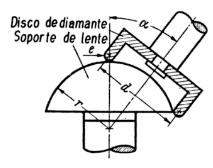
\includegraphics[width=150px]{c:/Users/Inventor/Documents/GitHub/Scripts/Python Scripts/Angulo Generado Superficies Opticas/Angulo_de_generado_superfices_opticas.png}%
\caption{Representacion de la relacion entre el diametro del disco de diamante, el radio de la lente y el angulo de ataque}%
\end{figure}

%
\end{document}